%-------------------------------------------------------------------------------
\section{Introduction}
%-------------------------------------------------------------------------------

Web applications today own, store, and sell user data, often without the user's knowledge or
explicit consent~\cite{nytimes:fb, npr:data}. This has dangerous consequences for both users and
application developers, as data leaks lead to loss of livelihoods and lawsuits~\cite{breach:twitter,
breach:fb, breach:marriott, breach:quora}. Granting web applications complete ownership
of personal data clearly fails to protect users' privacy. 

However, a world in which the user has complete data ownership is equally problematic. Although
theoretically feasible~\cite{amber, w5, blockstack, bstore}, this model results in an arguably even
less desirable world for users. 
%
Applications compute on per-user, filesystem-esque storage and run as JavaScript in users' browsers,
becoming slow and limited. Applications lose the flexibility and ease of programming over SQL
databases with application-specific schemas, and each user must implement the proper access control
and authentication mechanisms for data sharing.  As a result, service-side computation and data
sharing between users---a large reason users use applications to begin with---becomes cumbersome.
Furthermore, users are burdened with long-term data maintenance and storage: solutions that use PKI
(\eg Blockstack~\cite{blockstack}) require users to maintain a master private key, a cumbersome and
fragile solution in which losing the key results in permanent loss of all the user's data.
%
Finally, users must change the way they pay for services, as the current revenue model for
applications relies on access to user data. 
\lyt{this might not be a bad thing, though}.

This paper proposes a new model of \emph{flexible data ownership} for web applications that balances
users' desire for privacy with their desire for application utility. In this model, users subscribe
to applications by granting a time-limited lease to their data, with the provision that the
application may retain only de-identified information once the user unsubscribes. Users flexibly
switch between a privacy-preserving unsubscribed mode and an identity-revealing subscribed mode at
any time without permanently losing their data. Applications can continue to operate using their
current web architecture, retaining their revenue model, performance and reliability, and utility
for their users. Applications do not need to access any removed unsubscribed users' data,
simplifying the storage of this data when users enter privacy-preserving mode.
Figure~\ref{fig:world} illustrates this flexible transfer of data ownership in our new model,
compared to the two extremes of complete user ownership and complete application ownership of user
data.

\begin{figure*}[ht!]
    \centering
    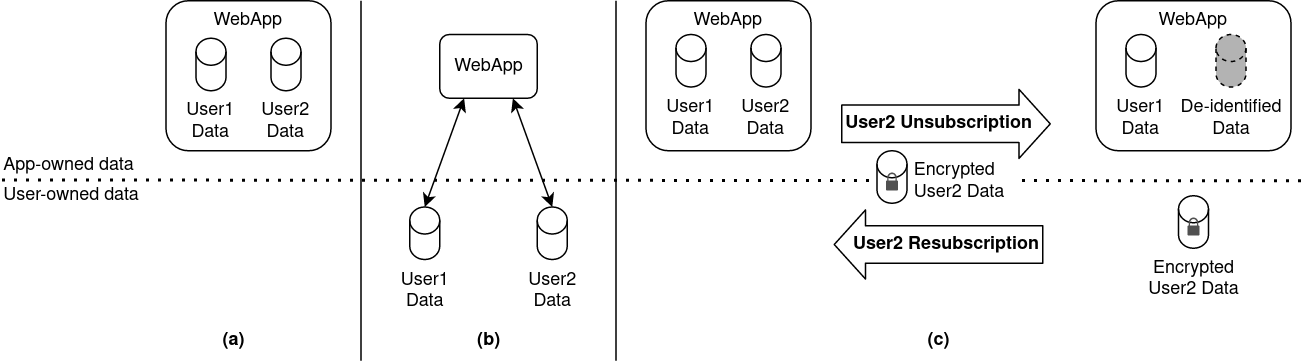
\includegraphics[width=\textwidth]{img/worlds}

    \caption{\textbf{(a)} The existing world of web applications, with applications maintaining and
    owning user data; \textbf{(b)} A world in which users have complete ownership of their data in cloud or local
    storage, and grant applications access to their data;
    \textbf{(c)} Our proposed model, which allows users to switch between privacy-preserving unsubscribed
    mode (right) and identity-revealing subscribed mode (left).}
    \label{fig:world}
\end{figure*}

This model clearly benefits the user: they can choose privacy at any time, without permanently
losing their accounts or affecting the utility of the applications for others.  But more
importantly, the model benefits application developers as well. Recent laws such as the European
Union's General Data Protection Regulation (GDPR)~\cite{eu:gdpr} and California's Consumer Privacy
Act (CCPA)~\cite{ca:privacy-act} codify users' rights to data ownership, granting users the right to
request erasure of information related to them. This model enables applications to comply with these
legal mandates, while still allowing its departing users to easily come back: if applications must
let users leave, it is in their best interest to make it easy for them to return. Furthermore,
applications optimize the amount of data available to generate profit and provide utility for
subscribed users, since they retain use of subscribed users' data, and de-identified data of
unsubscribed users. Because the application holds only identifying data for currently subscribed
users, this reduces the amount of compromising data in the system to only those users who have
actively agreed to temporarily give up their privacy.

However, even with legal incentives in place, this model is far from realized. Unsubscription is
often impossible or cumbersome (users often contact the developers or customer support directly in
order to unsubscribe)~\cite{jdm}, and developers manually implement coarse-grained, error-prone, and
often incomplete unsubscription that fails to completely de-identify the user. Even worse, no existing
application (to our knowledge) supports privacy-preserving unsubscription with the possiblity of
resubscription.  Application unsubscription thus permanently deletes years or even decades of
accumulated application data, costing both users and the web application, and creating little
incentive for the application to support easy unsubscription. 

In order to make flexible data ownership possible, we must solve the many
challenges faced by application developers. Key among these are the requirements to
selectively retain unsubscribed users' data for legal or application purposes while properly
de-identifying this data, and to allow the user to resubscribe at any time to their last-known
subscribed state. The complex data transformations required by user unsubscription and
resubscription highlight the need for new tools that allow developers to easily and systematically
automate the process.

%In the rest of this paper, we describe in more detail the state of unsubscription and resubscription in
%web applications today, and the challenges of implementing it correctly.  We then present \sys, a
%system that provides abstractions and mechanisms to help developers of databased-backed web
%applications achieve correct, privacy-compliant user unsubscription and resubscription without
%onerous labor, and without adding undue overheads.
